% Dokumentenklasse definieren
\documentclass[12pt]{article}

\usepackage{packages/general-packages}
\usepackage{config/config}


% Kopf- und Fußzeile
\lhead{}
\lfoot{}
\rhead{}
\rfoot{Zuo haftet für schlechte Noten}



%? Einfügen eines Inhalts-, Tabellen- und Grafikverzeichnisses
%* Bei Bedarf unbenötigte Verzeichnisse auskommentieren

\pagenumbering{arabic}

%\chead{}
%\rhead{}
\cfoot{\thepage \hspace{1.5mm} $|$ \hspace{0.5mm} \pageref{LastPage}}

\raggedright

% Inhaltsverzeichnis
%\tableofcontents

% Abbildungsverzeichnis
%\listoffigures

% Tabellenverzeichnis
%\listoftables




\begin{document}

\section{Leitungen und Netze}
\subsection{Bauformen}
\subsubsection{Betriebsgrößen, Begriffe}
\begin{enumerate}
    \item \textit{Welche Spannungsebenen werden in der elektrischen Energieübertragung unterschieden: 
    Nennen Sie die Spannungsbereiche und die jeweilige Anwendung.}\\
    \begin{table}[!ht]
        \centering
        \begin{tabularx}{\textwidth}{|l|l|X|}
        \hline
            Spannungsbereich & Nennspannung  & Anwendung  \\ \hline
            Niederspannung & Bis 1kV, typisch 400V & Kleinverbraucher und Haushalte, Lokal, Photovoltaik   \\ \hline
            Mittelspannung &  typisch (3/6/10/15/20/30) kV & Großabnehmer, Stadtversorgung, Regional  \\ \hline
            Hochspannung &  typisch (60/110) kV & Stadt- und Überlandversorgung, Überregional  \\ \hline
            Höchstspannung &  typisch (220/380/500/700) kV & Großraumversorgung, Verbundwirtschaft, International  \\ \hline
        \end{tabularx}
    \end{table}
    
    \item \textit{Welchem Spannungsbereich wird die Nennspannung 110kV zugeordnet?}\\
    Hochspannung
    
    \item \textit{Welchem Spannungsbereich wird die Nennspannung 60kV zugeordnet?}\\
    Hochspannung

\end{enumerate}


\subsubsection{Kabel}

\begin{enumerate}
    \item \textit{Warum werden bei höheren Spannungen bevorzugt Einleiterkabel eingesetzt?}\\
    Die Abstände zwischen den Kabeln sind größer als bei Mehrleiterkabel $\rightarrow$ kleinere elektrische Felder
    \clearpage
    \item \textit{Radialfeldkabel, Gürtelkabel: Beschreibung, Skizze}\\
    \begin{figure}[h]
        \includegraphics[width=\textwidth]{figures/Gürtelkabel.PNG}
        \centering
    \end{figure}

    \begin{figure}[h]
        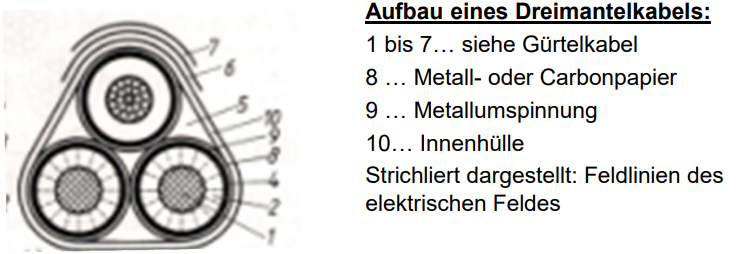
\includegraphics[width=\textwidth]{figures/Radialfeldkabel.PNG}
        \centering
    \end{figure}

    \item \textit{Skizzieren und beschreiben Sie den Aufbau eines Radialfeldkabels. Zeichnen Sie in die Skizze die Feldlinien des elektrischen Feldes ein zu einem Zeitpunkt t mit 
    U1(t)=Scheitelwert von U und U2(t)=U3(t)=-1/2*Scheitelwert von U}\\
    • Einsatz für höhere Spannungen möglich\\
    • Dreimantelkabel von 15kV bis 30kV; Einleiterkabel bis 60kV (kleinere Durchmesser bei diesem Ausmaß)\\
    • Der radialsymmetrischen Feldverlauf wird durch die einzelnen Leiterisolierungen mit Metallpapier 
    (Hochstädter-Kabel) erreicht, während beim Mehrmantel- oder Dreimantelkabel jeder Leiter von einem eigenen 
    Metallmantel umgeben ist\\
    • Größte Flussdichte und Feldverzerrung des elektrischen Feldes tritt an der Oberfläche des mehrdrähtigen 
    Leiters auf\\
    • Leitfähigen Papierlagen oder Kunststoff zwischen Leiter und Aderisolierung für gleichmäßigen Feldverlauf\\
    \clearpage
    \item \textit{Skizzieren und beschreiben Sie den Aufbau eines Gürtelkabels. Zeichnen Sie in die Skizze die 
    Feldlinien des elektrischen Feldes ein zu einem Zeitpunkt t mit U1(t)=Scheitelwert von U und U2(t)=U3(t)=-1/2*Scheitelwert von U}\\
    • Einsatz bis 10kV\\
    • Elektrische Feld verläuft durch die durchschlagsfeste Leiterisolierung und verbleibenden Zwickel. Trotz Befüllung der Zwickel mit durchschlagsfester Leiterisolierung verbleiben Hohlräume, in welcher bei zu hoher Leiterspannung Teilentladungen auftreten und mit der Zeit zur Zerstörung der Leiterisolierung führen
    \\• Isoliermaterial: Ölgetränktes Papier\\
    \item \textit{Nennen Sie Gründe für die zunehmende Verwendung von kunststoffisolierten Kabeln.}\\
    PVC (Polyvinylchlorid – bis zu 10kV)
    • nicht hygroskopisch, auf Metallmantel kann dadurch verzichtet werden\\
    • Gute chemische Beständigkeit\\
    • Geringes Gewicht, biegsam\\
    • Durchschlagsfest \\
    • Verhältnismäßig große dielektrische Verluste\\
    
    VPE (Vernetztes Polyäthylen – bis zu 400kV)\\
    • Vorteile wie PVC\\
    • Geringe dielektrische Verluste\\
    • Sagenhafte thermische Eigenschaften\\
    \item \textit{Was versteht man unter "Massekabel" und welche 
    Vor- und Nachteile sind hierbei zu berücksichtigen?}\\
    Kabeln, bei der die Leiterisolierung aus mehreren Lagen Papier besteht, die mit Isolieröl getränkt wird\\
    Vorteile:\\
    • Geringe dielektrische Verluste\\
    Nachteile: \\
    • Gefahr von Teilentladungen durch Hohlraumbildung und Abwanderung von Tränkmasse; Schutz durch aufwändige Kabelverschlüsse und Verlegevorschriften (keine senkrechte Verlegung!)\\
    • Hygroskopische Eigenschaft\\
    • Starr, schwer zu verlegen\\
    • Schwer\\
    \item \textit{Welches Isoliermaterial wird gegenwärtig 
    vorwiegend in Kabeln von Mittel- und 
    Hochspannungsnetzen eingesetzt und welche 
    Vorteile bietet es gegenüber Massekabeln?}\\
    Kunststoffisolierung aus VPE  \\
    (Vorteile siehe Fragestellung 7)
    

    \item \textit{Welche Ursachen führen zur Hohlraumbildung in 
    einer Isolation bei Massekabeln? Was kann man 
    dagegen vorsehen?}\\ 
    Tränkmasse wandert ab, weil das Kabel zu steil verlegt wird. \\
    Kabel müssen streng nach Vorschrift verlegt werden, spezielle Endverschlüsse mit vorbehaltener Tränkmasse, welche in das Massekabel nachfließen kann.

    \item \textit{Welche Gefahr entsteht durch die Bildung von 
    Hohlräumen in der Isolation von Kabeln?}\\
    • Die Isolationsfähigkeit ist nicht mehr gegeben, es kann zu Durchschlägen kommen \\
    • Schlechtere thermische Eigenschaften, da Luft sich bei 
    Wärme ausdehnt kann weiteres Ölgemisch vertrieben werden oder eine der darüberliegenden Schicht beschädigt werden.\\
    \\• Ein erhöhter kapazitiver Effekt tritt auf
    \item \textit{Warum werden in Steilhängen bevorzugt 
    kunststoffisolierte Kabel eingesetzt?}\\
    Bei Massekabeln würde die Tränkmasse abwandern. Weiterhin haben Kunststoffkabel eine höhere Flexibilität, niedriges Gewicht, bessere chemische Beständigkeit etc.
    \item \textit{Warum werden papierisolierte Kabel mit einem 
    Mantel aus Blei oder Aluminium ausgerüstet?}\\
    Dadurch kann man eine gleichmäßige Feldverteilung erzielen.
    \item \textit{Was versteht man unter Dielektrizitätsverlusten bei 
    Hochspannungskabeln und wie sind diese bei der 
    Auswahl der Kabel für die jeweilige 
    Energieübergragung zu berücksichtigen? }\\
    Die ständige Umpolung der ortsfesten elektrischen Dipole in der Isolation, durch das elektrische Feld, 
    bei Wechselspannung erzeugt eine Erwärmung. \\
    Kabelauswahl: \\
    • PVC bis 10kV \\
    • VPE bis 400kV \\
    \item \textit{Welche el. Größe (Strom, Spannung) ist für die 
    Dielektrizitätsverluste hauptverantwortlich}\\
    Die Größe der Dielektrizitätsverluste ist abhängig von der Spannung und der dielektrischen 
    Verlustzahl des Isolierstoffs.
\end{enumerate}




\subsubsection{Kabelerwärmung}

\begin{enumerate}
    \item \textit{Welche elektrischen Verluste eines Kabels in Mittel und Hochspannungsnetzen führen zur 
    Dauererwärmung? }\\
    Dielektrizitätsverluste
    \item \textit{Gehören Dielektrizitätsverluste zu den 
    Stromwärmeverlusten? (Ja oder Nein, Begründen 
    Sie ihre Antwort)}\\
    Nein. Die Stromwärmeverluste wird durch den Stromfluss im Leiter aufgrund der Verlustleistung im wirksamen 
    Leiterwiderstand Erwärmung hervorgerufen, während die Dielektrizitätsverluste durch die ständige Umpolung 
    der ortsfesten elektrischer Dipole in der Isolation durch das elektrische Feld bei Wechselspannung 
    Erwärmung hervorgerufen wird. 
    \item \textit{Welche Widerstände sind bei der Berechnung der 
    Stromwärmeverluste eines Kabels in Mittel- und 
    Hochspannungsnetzen zu berücksichtigen?}\\
    Gleichstromwiderstand R und dem Zusatzwiderstand $\Delta$R (aus Skineffekt und Mantelverlusten)
    $R_W = R + \Delta R, R= \rho \cdot l / A, \Delta R \dots $aus Tabelle

    \item \textit{Welche Belastungen sind bei der Dimensionierung 
    von Kabeln hinsichtlich Wärmebeständigkeit zu 
    berücksichtigen? 
    (Erklären Sie zu jeder genannten Belastung jeweils 
    kurz die Ursache dieser Belastung)}\\
    Dauerbelastbarkeit: \\
    • Durch den Betriebsstrom im Normalbetrieb – Stromwärmeverluste/Dielektrizitätsverluste \\
    Kurzerwärmung: \\
    • durch einen Überstrom oder Kurzschluss bis zur Abschaltung des Überstromschutzorgans und daraus 
    hervorgerufener Stromwärmeverluste\\

    \item \textit{Was versteht man unter dem „Skineffekt“ bei einer 
    Energieübertragungsleitung und wie wird er in der 
    Berechnung berücksichtigt?}\\
    Sie ist ein physikalisches Phänomen, das in elektrischen Leitern, insbesondere bei hohen Frequenzen, auftritt. 
    Er führt dazu, dass elektrischer Strom dazu neigt, an der Oberfläche des Leiters zu fließen, 
    anstatt gleichmäßig im gesamten Querschnitt des Leiters verteilt zu werden. 
    Der Skineffekt wird in der Berechnung durch $\Delta$R berücksichtigt. 


    \item \textit{Was versteht man unter „Mantelverlusten“ bei 
    Kabeln und wie werden sie in der Berechnung 
    berücksichtigt?}\\
    Mantelverluste bezieht sich auf Verluste, 
    die in einem elektrischen oder elektronischen System auftreten, 
    wenn Wirbelströme im Metallmantel oder Bewehrung entstehen.
    Die Mantelverluste werden gleich wie die Verluste durch den Skineffekt durch $\Delta$R beschrieben.


\end{enumerate}

\subsubsection{Freileitung}


\begin{enumerate}
    \item \textit{Welche Aufgabe hat das Erdseil bei Freileitungen?}\\
    Blitzschutz, Verbindung der Erder aller Masten (Potenzialausgleich)
    \item \textit{Wie erfolgt die Masterdung bei Freileitungsmasten, 
    wozu dient die Masterdung?}\\
    Als Erder werden Ring- oder Strahlenförmig in Erde verlegte Bandeisen oder tief in das Erdreich eingetriebene 
    Tiefenerder verwendet. \\
    • Erd- und Erdkurzschlussströme durch Isolatorüberschlag abzuleiten\\
    • Erd- oder Blitzschutzseil mit der Erde zu verbinden\\
    \clearpage
    \item \textit{Wie ist der Blitzschutzraum bei Freileitungsmasten 
    definiert}\\
    
    \begin{figure}[h]
        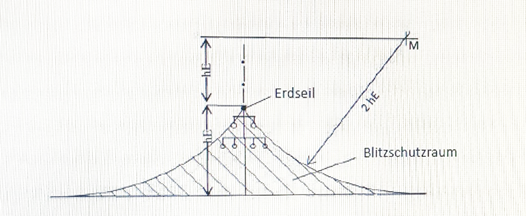
\includegraphics[width=\textwidth]{figures/Blitzschutzbereich.png}
        \centering
    \end{figure}
    \item \textit{Welche Maßnahmen werden bei Freileitungen 
    verwendet, um Teilentladungen (Korona) durch zu 
    hohe Randfeldstärke zu vermeiden?}\\
    • Querschnittvergrößerung (bei Mittel- und teilw. Hochspannungsleitungen)\\
    • Bündelleiter\\
    \item \textit{Warum und unter welchen Bedingungen werden 
    Freileitungen als Bündelleiter ausgeführt?}\\
    Durch Bündelleiter können Teilentladungen, die durch zu hohe Randfeldstärken entstehen, vermieden werden. Dadurch lassen sich Probleme wie Störgeräusche, 
    elektromagnetische Störungen und Verlustleistungen beseitigen. Bevorzugt bei Hoch- und Höchstspannung.
    \item \textit{Welche Aufgabe haben die Lichtbogenarmaturen 
    an Isolatorketten von Freileitungen?}\\
    Sie erfüllen die Aufgaben: \\
    • Verbinden von Mast, Seil und Isolatoren \\
    • Lichtbogenschutz: Um bei Isolatorüberschlag die Glimmentladung und den Lichtbogen vom Porzellan fernzuhalten \\
    \item  \textit{Was ist bei der Wahl der Aufhängungspunkte und 
    des Durchhanges zu beachten?}\\
    Der Seildurchhang ist so einzustellen, dass die Höchstszugspannung in den Aufhängepunkten auch bei 
    klimatischen Grenzbedingungen (Windlast, Temperatur, Eislast) nicht erreicht wird. Die Abstände der Leiter 
    zueinander sowie zwischen Leiter und geerdeten Teilen (z.B. Mast, Traverse) muss so groß sein, 
    dass bei Schwingen durch Wind ein Zusammenschlagen oder eine Annäherung bis zum Überschlag nicht erfolgt. 
    Schutz vor zufällige Berührung: \\
    • UN = 110kV: Abstand zum Erdboden >= 6m \\
    • UN = 220kV: Abstand zum Erdboden >= 6,75m \\
    • UN = 380kV: Abstand zum Erdboden >= 7,8m


\end{enumerate}

\subsection{Berechnungen}
\subsubsection{Leitungsnachbildung}

\clearpage

\begin{enumerate}
    \item \textit{Zeichnen Sie das vereinfachte einphasige 
    Ersatzschaltbild einer symmetrisch betriebenen 
    Drehstromleitung mit konzentrierten 
    Längsimpedanzen}\\
    \begin{figure}[h]
        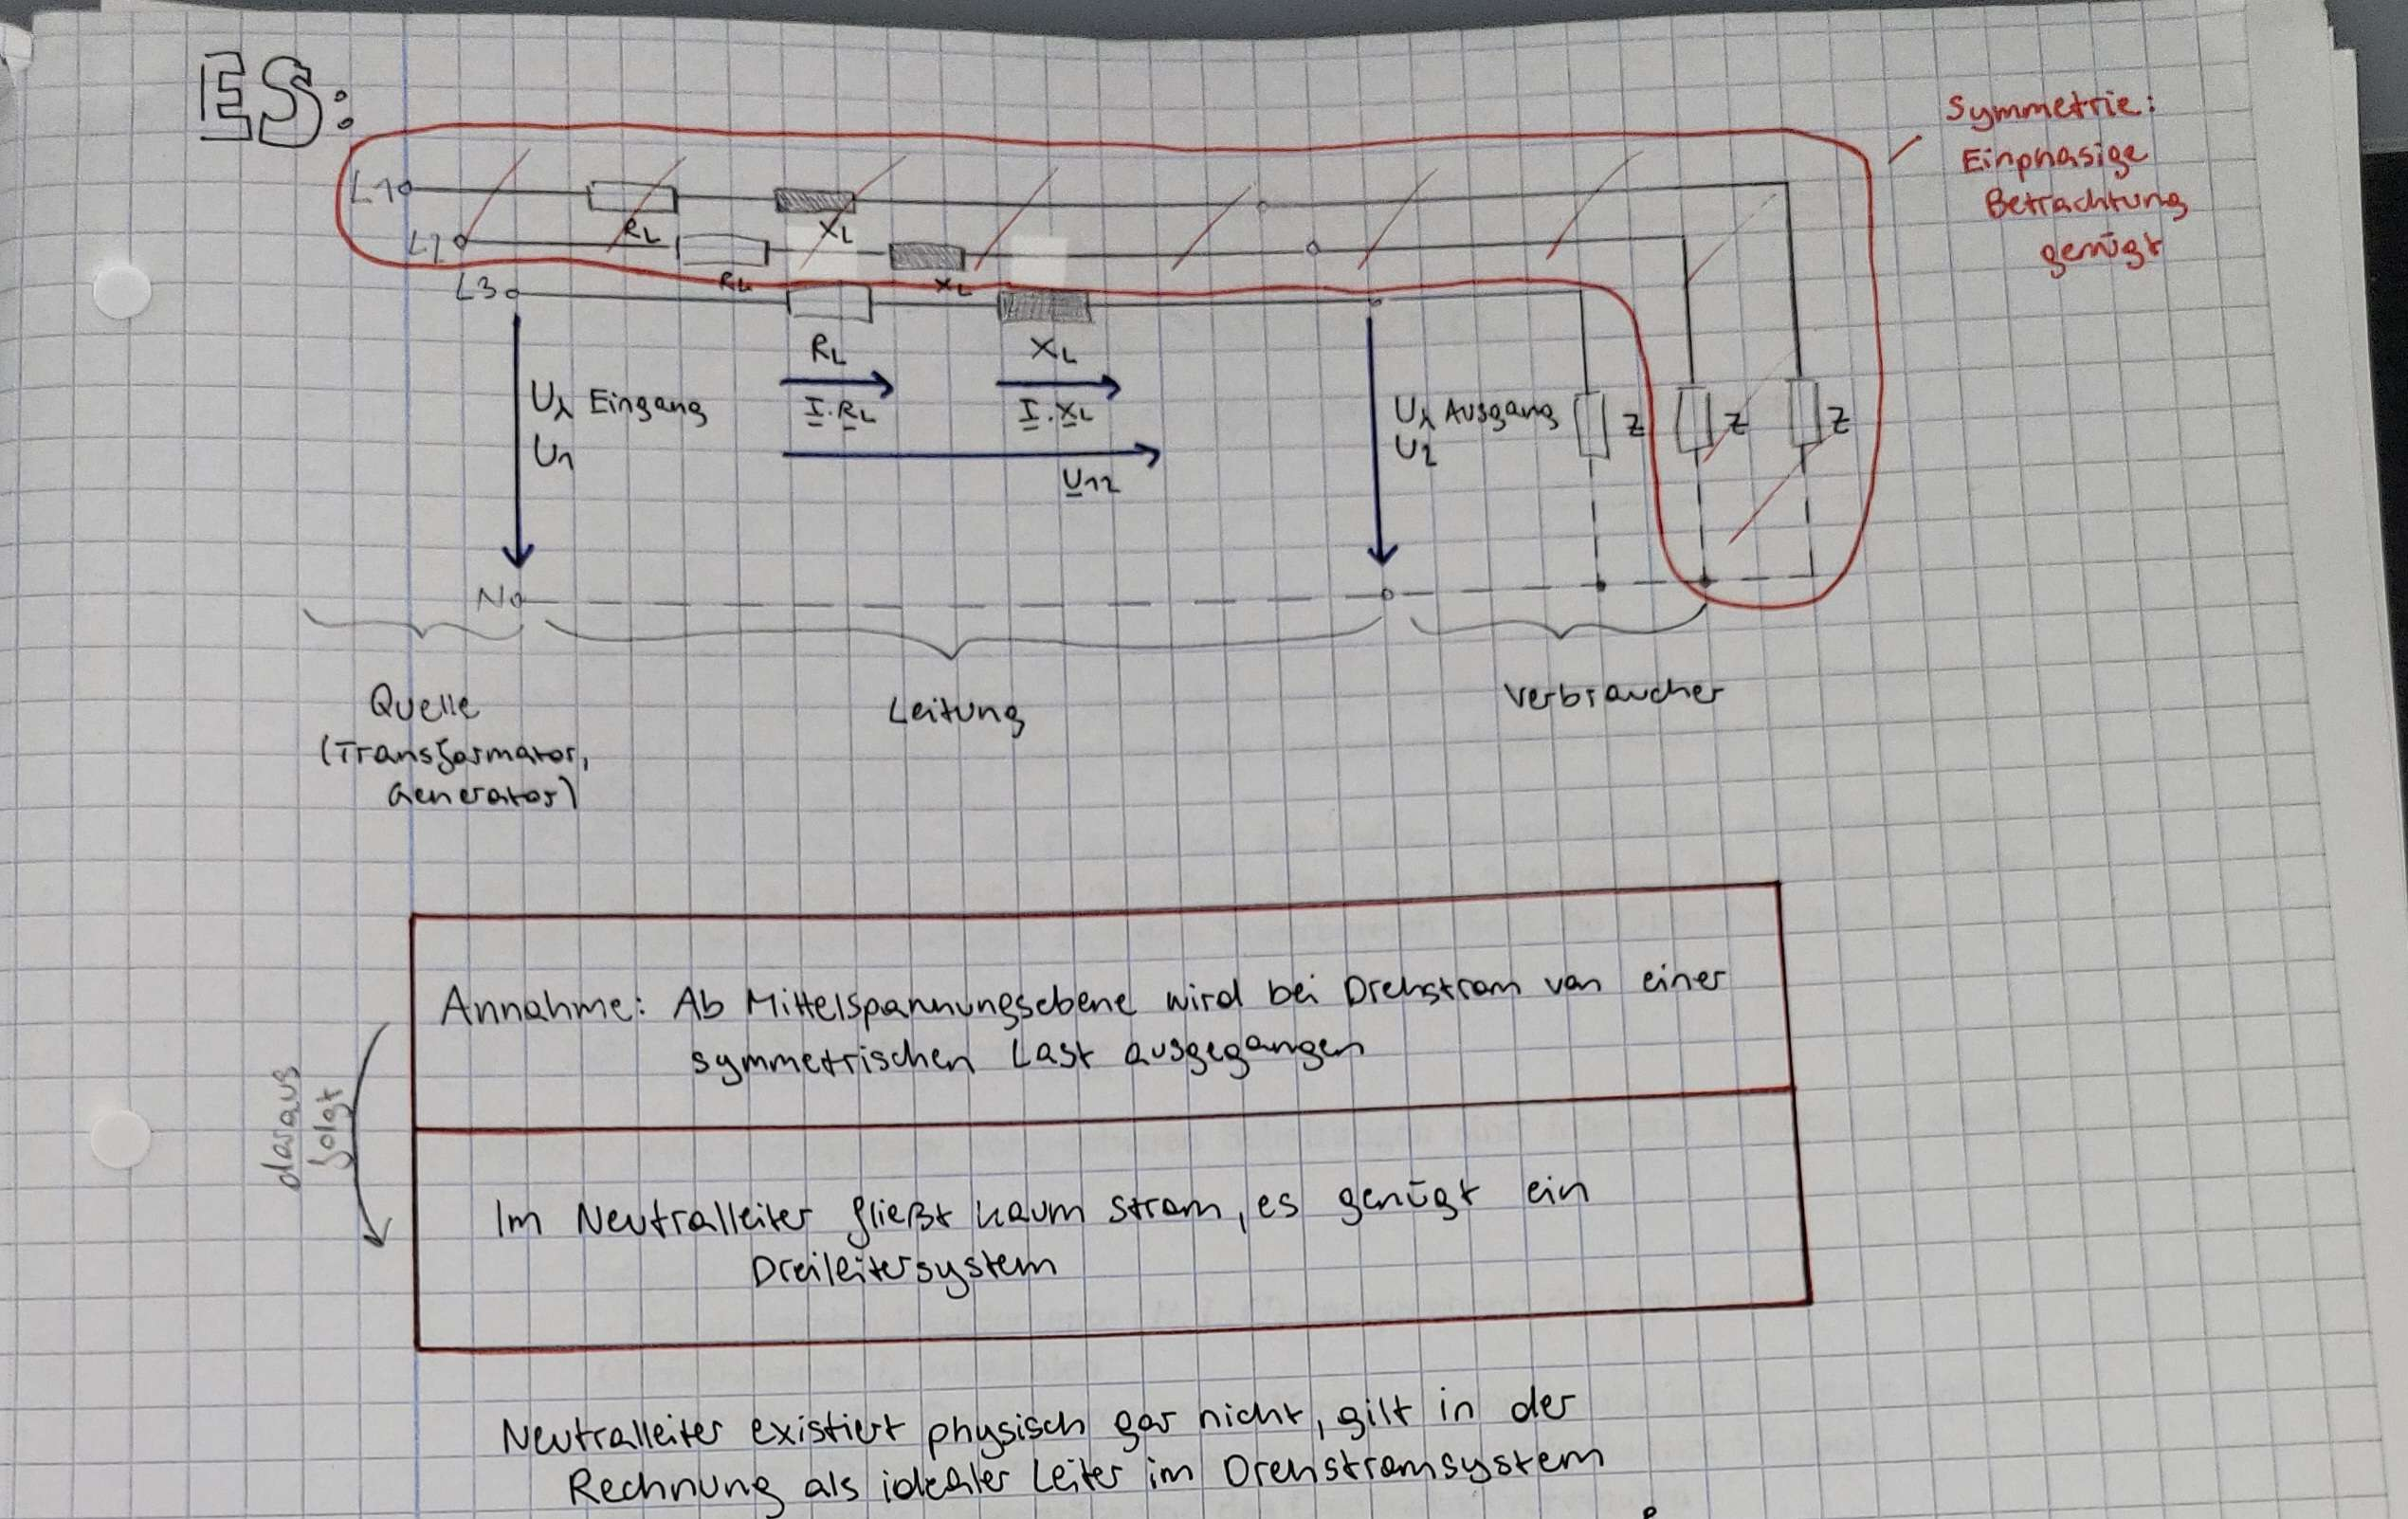
\includegraphics[width=\textwidth]{figures/Schaltbild.jpg}
        \centering
    \end{figure}
    \clearpage
    \item \textit{Zeichnen Sie das einphasige Ersatzschaltbild einer 
    symmetrisch betriebenen Drehstromleitung mit 
    konzentrierten Längsimpedanzen und der 
    Queradmittanz konzentriert am Leitungsende (T-Halbglied)}\\
    \begin{figure}[h]
        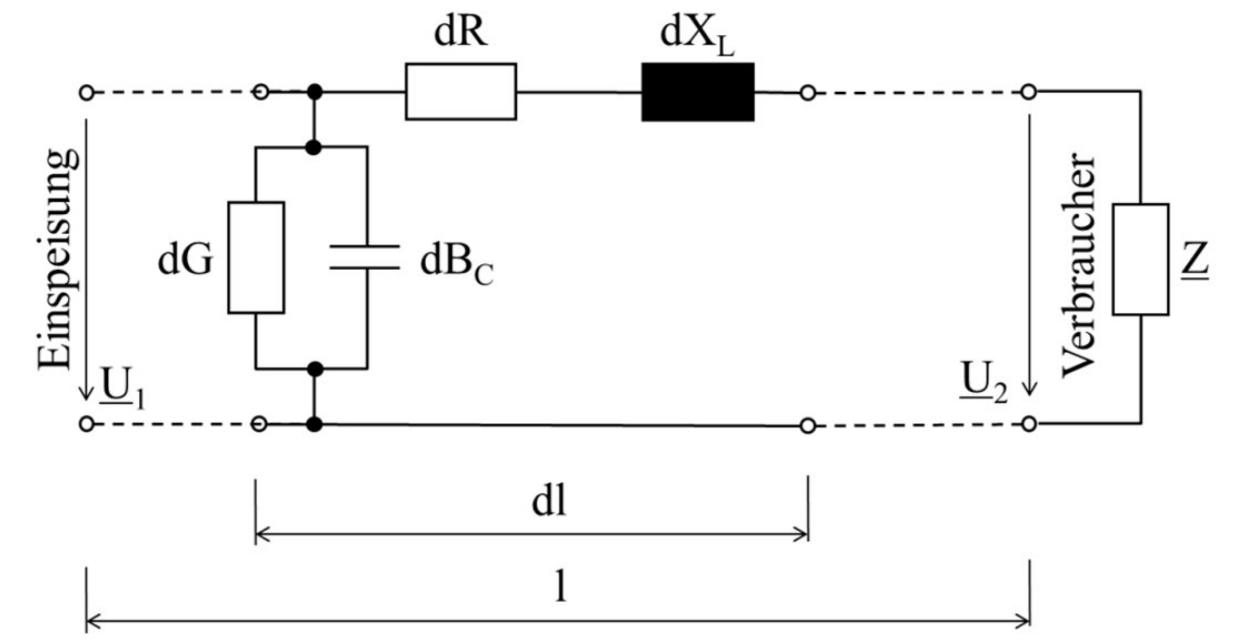
\includegraphics[width=\textwidth]{figures/T-Halbglied.PNG}
        \centering
    \end{figure}
    \clearpage
    
    \item \textit{Zeichnen Sie das einphasige Ersatzschaltbild einer 
    symmetrisch betriebenen Drehstromleitung mit 
    konzentrierten Längsimpedanzen und der 
    Queradmidanz konzentriert am Leitungsanfang und -
    ende (II-Glied)}\\

    \begin{figure}[h]
        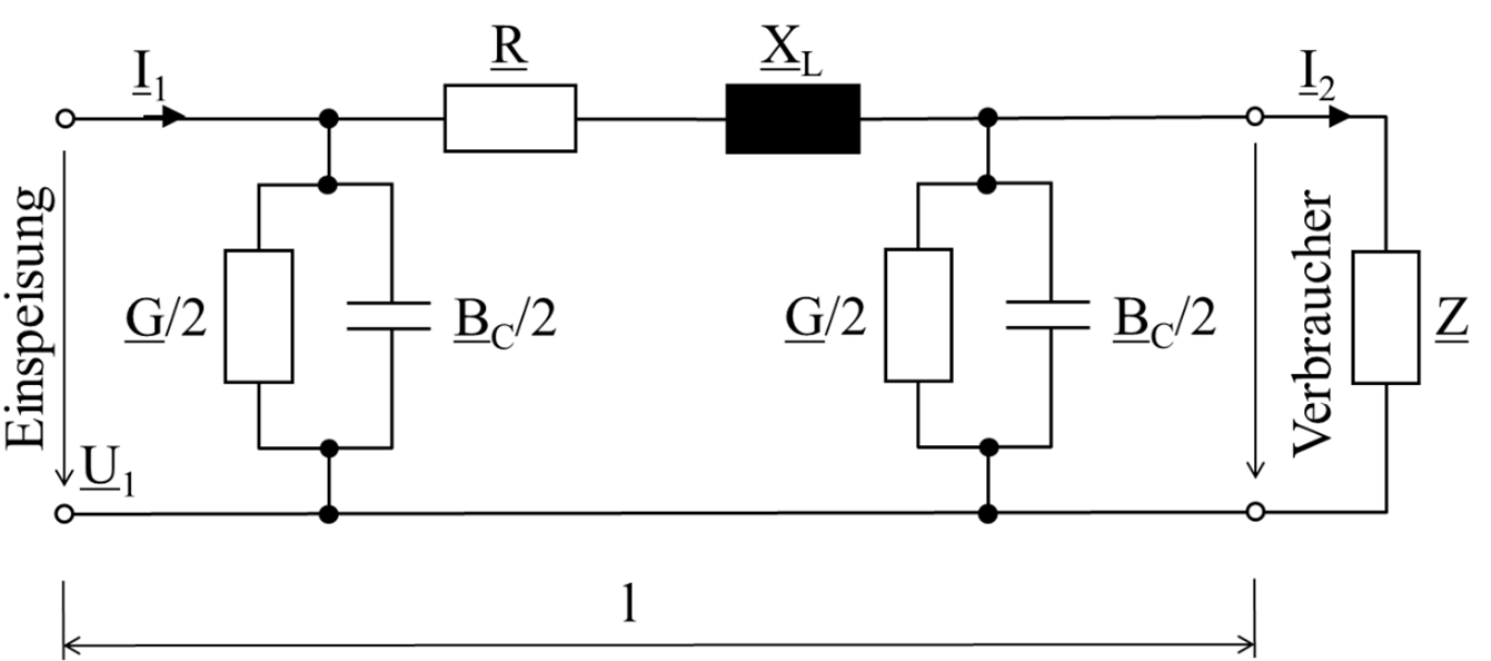
\includegraphics[width=\textwidth]{figures/II-Glied.PNG}
        \centering
    \end{figure}

    \item \textit{Erklären Sie den Unterschied zwischen $\Delta$U und 
    U12 anhand des Zeigerdiagrammes eines Nieder- und Mittelspannungsnetzes für eine einseitig 
    gespeiste Leitung mit einer Abnahme}\\

    \begin{figure}[h]
        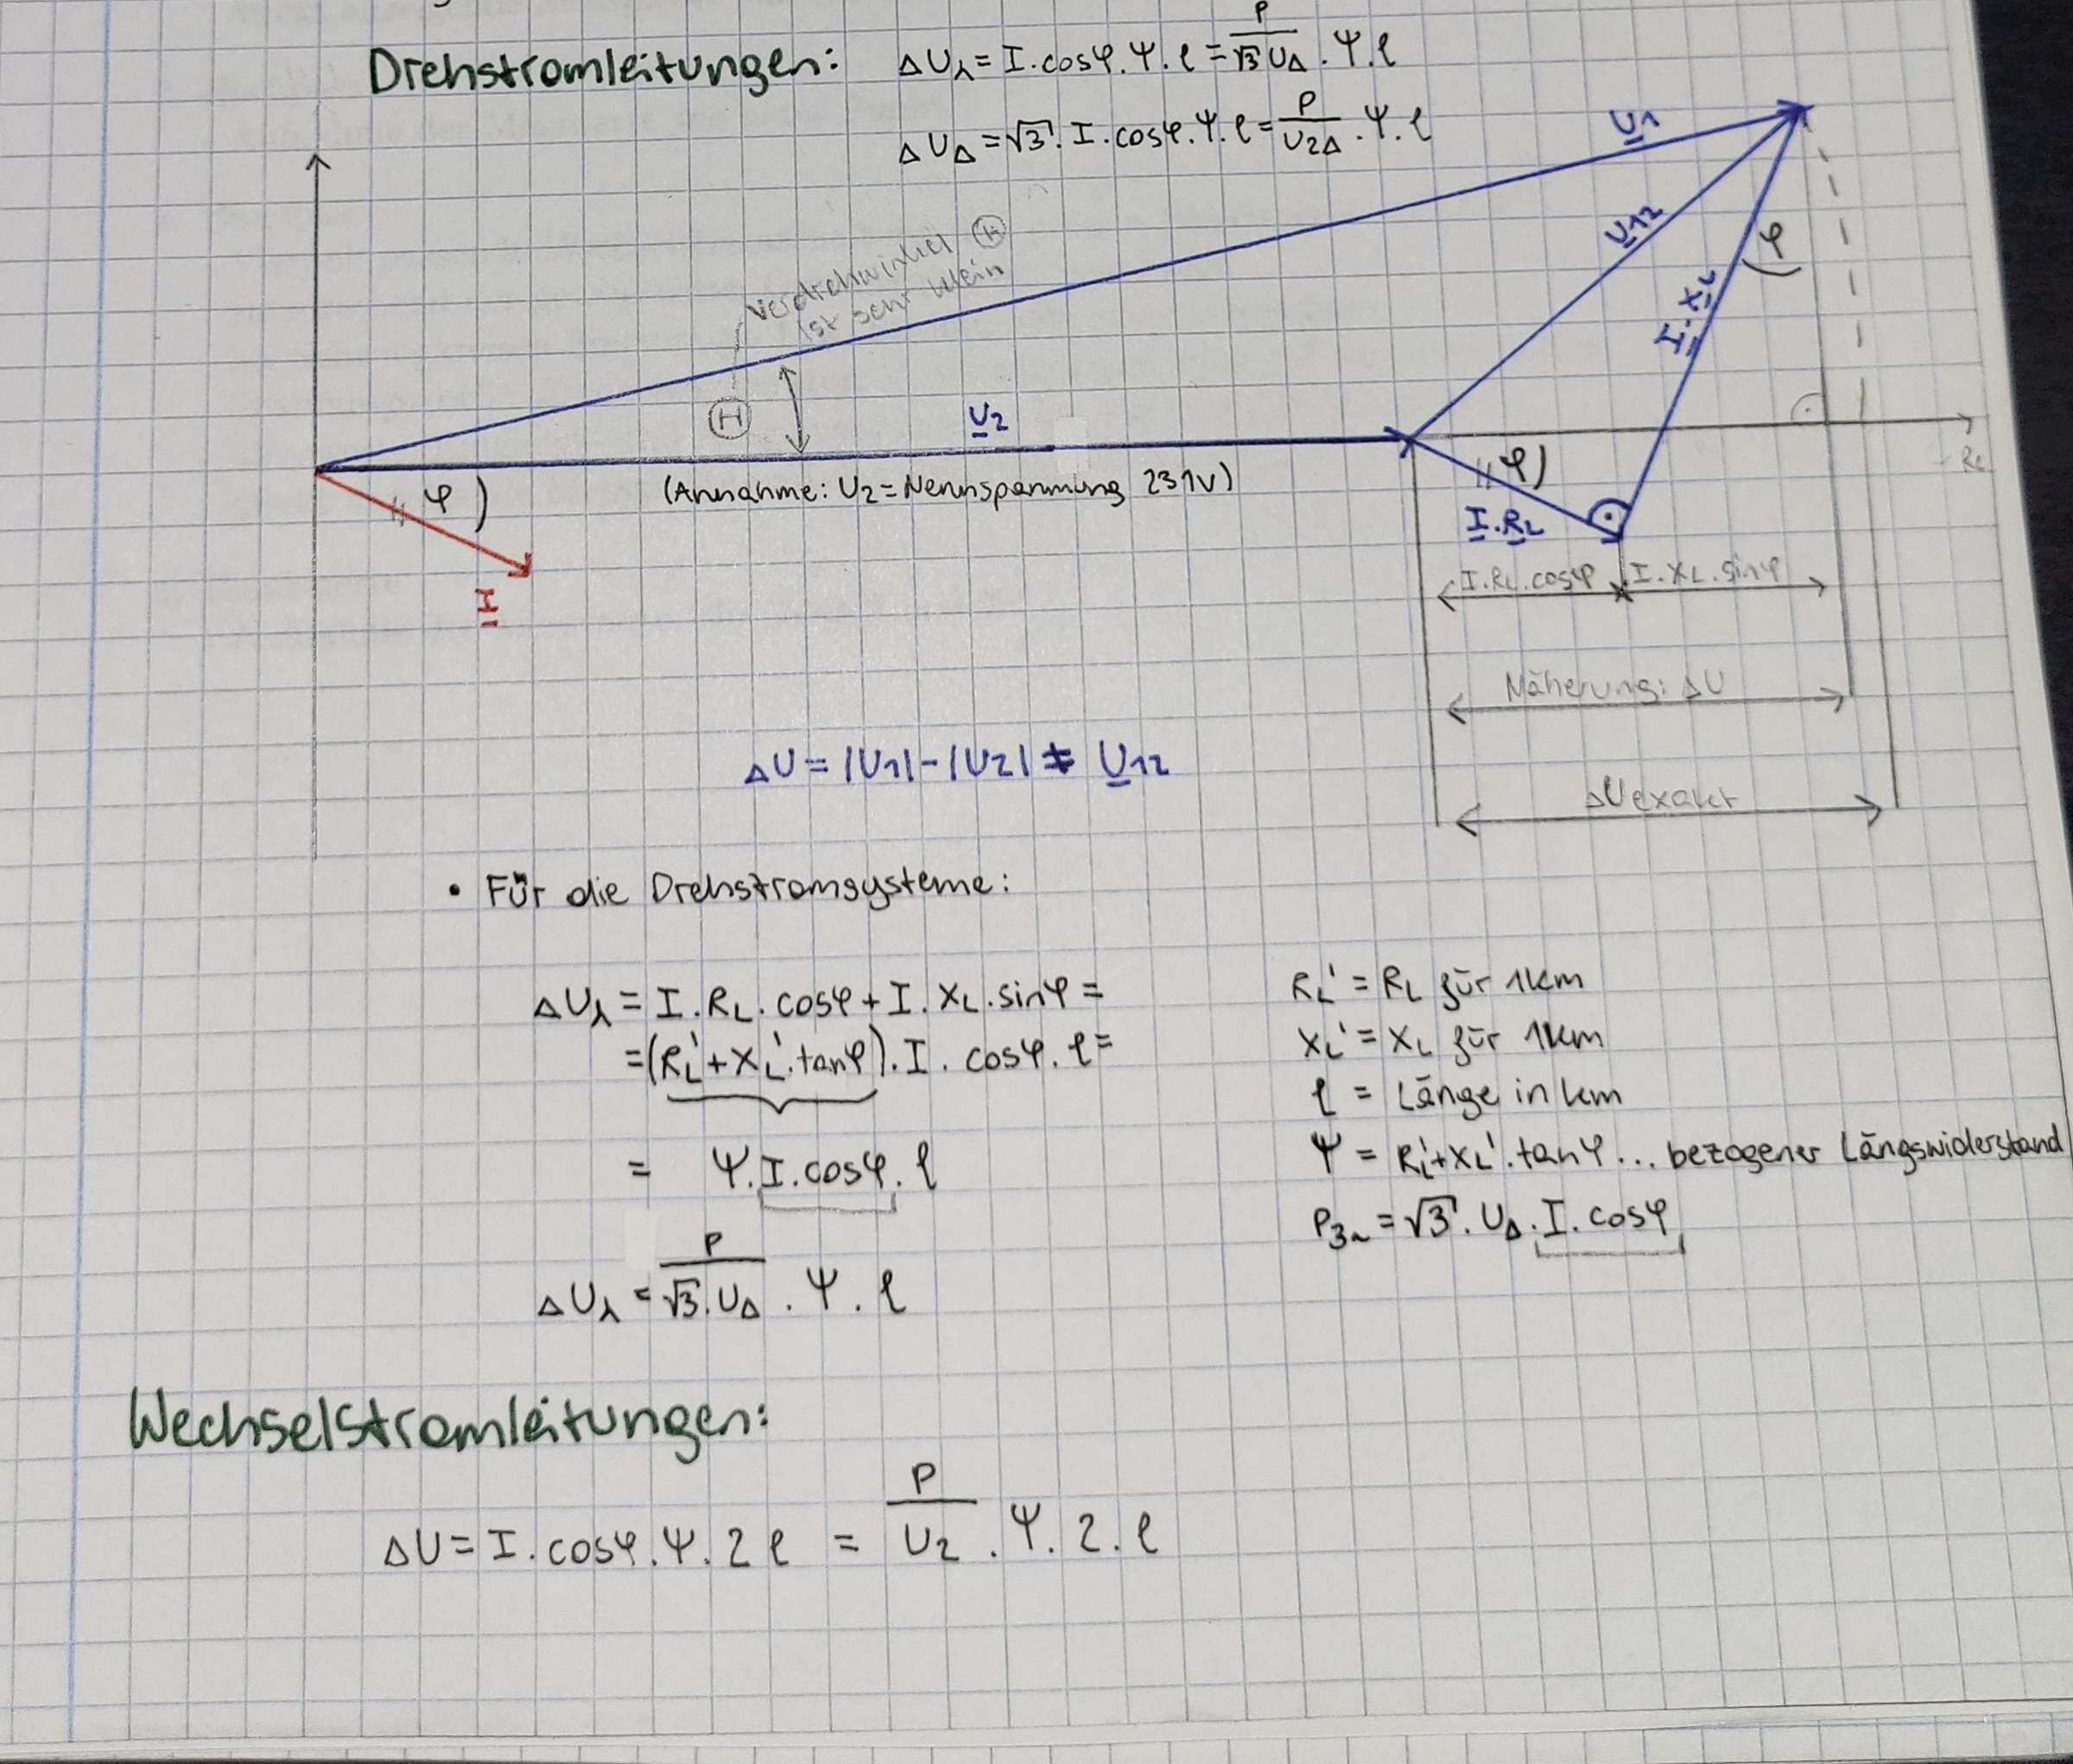
\includegraphics[width=\textwidth]{figures/Zeiger.jpg}
        \centering
    \end{figure}


    \item \textit{Was versteht man unter dem Widerstandsbelag 
    einer Leitung?}\\
    $R'$ in $\Omega / km$

    \item \textit{Weshalb besitzen elektrische Leitungen eine 
    Kapazität?}\\
    Leiterseile oder Erde sind wie die Elektroden eines Kondensators zu betrachten bzw. 
    sie sind Elektroden. Zwischen verschiedenen Leiterseilen und zwischen den Leiterseilen und der Erde wird Energie gespeichert.
    \item \textit{Unter welchen Bedingungen kann die 
    Leitungskapazität von Netzen vernachlässigt 
    werden, wann ist sie zu berücksichtigen?}\\
    Für elektrisch kurze Leitungen (Freileitungslänge unter 100km) und Betrieb bei 
    Normallast kann sowohl der Wirkleitwert G als auch die Betriebskapazität $B_C$
    vernachlässigt werden, sonst muss sie berücksichtigt werden.
    \item \textit{Unter welchen Bedingungen kann der Wirkleitwert 
    von Netzen vernachlässigt werden, wann ist sie zu 
    berücksichtigen?}\\
    Für elektrisch kurze Leitungen (Freileitungslänge unter 100km) und Betrieb bei 
    Normallast kann sowohl der Wirkleitwert G als auch die Betriebskapazität $B_C$
    vernachlässigt werden.
    \item \textit{Unter welchen Bedingungen kann es zu 
    Spannungserhöhungen am Ende einer Leitung 
    kommen?}\\
    Photovoltaik


\end{enumerate}





\subsection{Wirr-Warr vom freundchen Mühlbacher ohne wirkliche Fragen (eigentlich der Stoff + seine PDF + Zeugs das man wissen sollte, keine Ahnung)}



Einseitig gesp. Leitung mit einer Abnahme \\
Einseitig gesp. Leitung mit verteilter Abnahme \\
Einseitig gesp. Verzweigte Leitung \\
Zweiseitig gesp. Leitung \\
Vermaschtes Netz \\
(komplexe Lastflussber.) \\
Erd- und Kurzschluss \\
Sternpunktbehandlung \\
Sternpunktschaltung \\
Kurzschlussfestigkeit, \\
Überspannungsschutz, Isolationskoordination \\
Entstehung von Überspannungen \\
Schutzeinrichtungen gegen Überspannungen \\










\end{document}


